\chapter{数据链路层}\label{CN03}

\par\medskip\noindent\textbf{知识导图}\par\smallskip
\begin{wideblock}\centering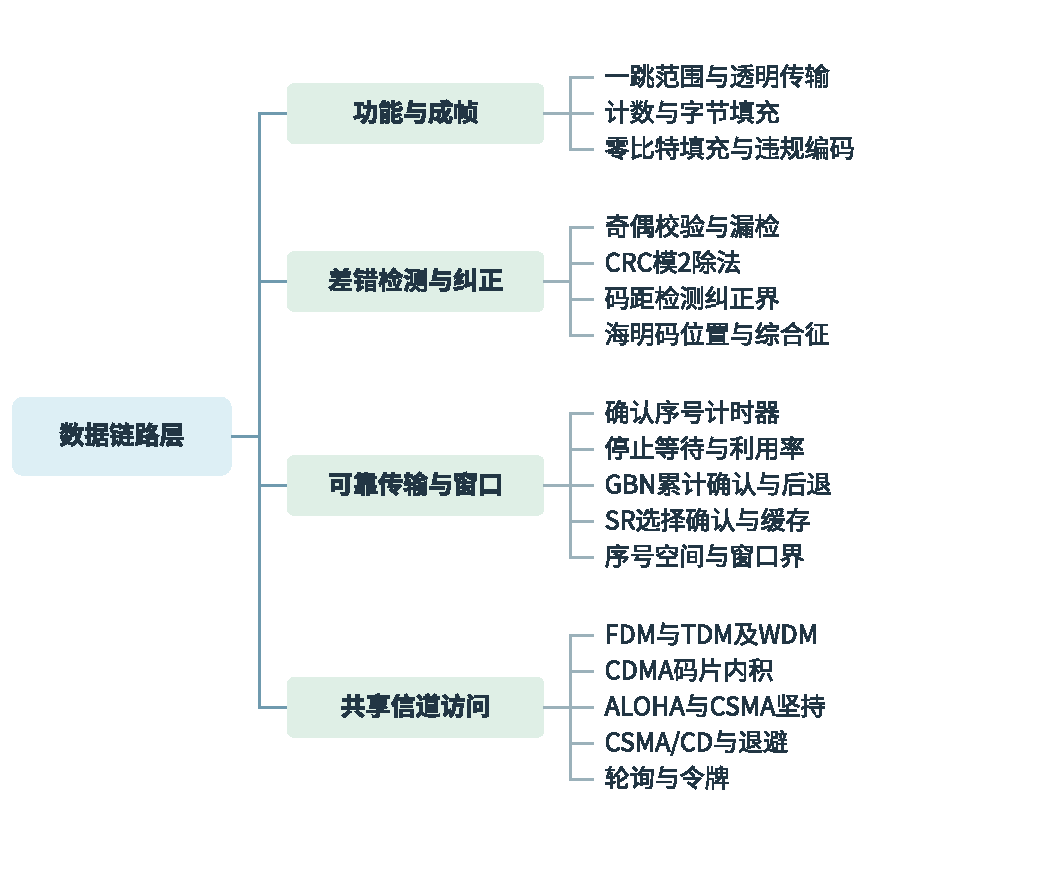
\includegraphics[width=\linewidth,height=168mm,keepaspectratio]{figures/map-01.pdf}\end{wideblock}\par\medskip\clearpage

\par\medskip\noindent\textbf{知识导图（续）}\par\smallskip
\begin{wideblock}\centering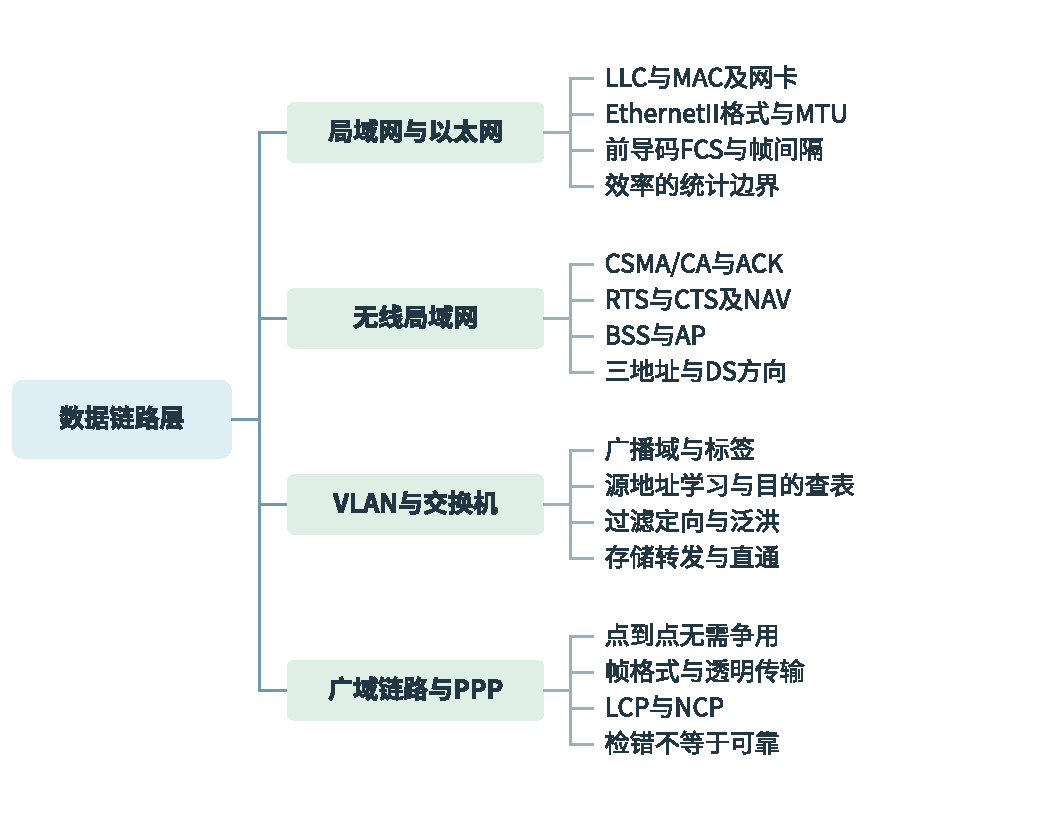
\includegraphics[width=\linewidth,height=168mm,keepaspectratio]{figures/map-02.pdf}\end{wideblock}\par\medskip\clearpage

数据链路层先解决``这一串比特属于哪一帧、有没有检测出错误''，再按协议决定是否确认和重传。若多个节点共用介质，还必须决定谁现在可以发送。这三类问题不能互相替代：CRC 不负责仲裁信道，介质访问成功也不保证帧已经可靠交付。

本章帧序号按模 \(2^k\) 循环。除题干另有约定，\texttt{ACK i} 表示``已正确收到 \(i\) 号帧''；TCP 的确认号采用``下一期待字节''，将在第5章单独说明。

\section{一跳链路提供什么功能}\label{CN03-01}

物理链路提供比特传输，数据链路在其上增加协议控制。基本任务包括成帧与透明传输、差错检测；具体协议还可能提供流量控制、确认重传、连接管理或共享介质访问控制。点到点链路不需要在多个竞争站之间分配介质，不能因此说它没有数据链路层。

\textbf{流量控制}协调发送速度与接收能力，防止接收缓存被压满；\textbf{差错控制}处理损坏、丢失、重复和次序问题。反馈窗口可以同时限制在途数据，既影响接收缓存需求，也影响重传管理。但只把发送器调慢一些，并不构成随接收状态变化的反馈控制。〖3.4-018〗

判断某项功能属于哪层，还要看范围。链路层确认只说明当前相邻节点的交付情况；路由器收到一帧后，下一跳仍可能丢失。端到端可靠性不能只由某一跳的 ACK 推出。

\section{怎样从连续比特中划出帧}\label{CN03-02}

\begin{definition}[帧边界与透明传输]

\textbf{帧定界}使接收方找到首尾，\textbf{透明传输}使任何合法上层数据都不会被误认为定界信息。主要方法的区别如下。

\end{definition}

\begin{wideblock}

\par\medskip\noindent\begin{minipage}{\linewidth}\fontsize{9.3}{12}\selectfont\begin{tabularx}{\linewidth}{@{}YYY@{}}
\toprule\noalign{}
\begin{minipage}[b]{\linewidth}\raggedright
方法
\end{minipage} & \begin{minipage}[b]{\linewidth}\raggedright
接收方怎样定位边界
\end{minipage} & \begin{minipage}[b]{\linewidth}\raggedright
必须处理的问题
\end{minipage} \\
\midrule\noalign{}


字符计数 & 读首部长度，再取相应字节 & 长度字段损坏可能使后续边界也错位 \\
字节填充 & 识别特殊定界字节 & 数据中的定界字节和转义字节都要转义 \\
零比特填充 & 识别 \texttt{01111110} 等标志 & 数据中每连续5个1后插0，避免形成标志 \\
违规编码 & 利用数据编码中不用的信号组合 & 依赖具体物理编码中确有可保留的组合 \\
\bottomrule\end{tabularx}
\end{minipage}\par\medskip

\end{wideblock}

字节填充必须按协议的转义规则执行。例如把数据中的 \texttt{FLAG} 写成 \texttt{ESC FLAG}、\texttt{ESC} 写成 \texttt{ESC ESC}，接收方遇到 \texttt{ESC} 时把后一个字节当作数据。若只转义 \texttt{FLAG}，原有 \texttt{ESC} 就会改变后续字节的解释。PPP 的具体异步字节转义还会改变被转义字节的数值，不能把所有字节填充都当成这一种简化写法。

零比特填充只扫描应填充的数据与控制区，不把首尾标志本身再填充。数据 \texttt{01111110} 中第五个连续1之后插0，成为 \texttt{011111010}；去填充时删掉这个插入0，恢复原数据。遇到恰好5个1，随后原数据还有一个0，线上会出现两个0，接收方只能删去填入的那一个。

\subsection{例 3-1　填充按连续1计数，不按字节重置}\label{CN03-ex1}

{\tcbset{SNbase/.append style={breakable=false}}\begin{example}[配套例题]

配套例题。 HDLC 协议对 \texttt{01111100 01111110} 组帧后对应的比特串为（　）。

A. \texttt{01111100 00111110 10}

B. \texttt{01111100 01111101 01111110}

C. \texttt{01111100 01111101 0}

D. \texttt{01111100 01111110 01111101}

\end{example}}

\textbf{解析。} 本题考查数据区的零比特填充；首尾标志不计入选项。原数据第一段中的5个连续1后插0，第二段的前5个1后也插0。连接原数据并逐位扫描，结果为 \texttt{011111000011111010}；按选项中的空格分组，所得结果与 A 相同，选 \textbf{A}。

空格只帮助阅读，并不表示连续1的计数在这里清零。本题借用 HDLC 背景说明填充机制，不要求另记该协议的完整控制字段。

\section{奇偶校验与 CRC：检验通过能推出什么}\label{CN03-03}

奇偶校验在数据后增加一位，使整个码字中1的个数满足奇数或偶数约定。任意奇数位翻转都会改变奇偶性，所以能够检测；偶数位翻转可能仍满足原奇偶性，无法保证发现。一个检验位不能指出是哪一位翻转，因此不具备单比特纠错能力。

\textbf{循环冗余检验 CRC}把比特串视为二元多项式。生成多项式 \(G(x)\) 的次数为 \(r\)，对应 \(r+1\) 位比特。发送数据 \(D\) 先左移 \(r\) 位，再按模2除法除以 \(G\)，余数 \(R\) 固定写成 \(r\) 位，发送 \(D\,R\)。模2减法就是逐位异或，不产生借位；最高位为0时也是如此。

以王道书§3.3算例的数据 \texttt{101001}、生成式 \texttt{1101} 为例，\(r=3\)，应计算 \texttt{101001000} 除以 \texttt{1101}。每次把除数首位对准当前最高1，异或后得到以下中间数：

\begin{codeblock}[language={}]
101001000
011101000  // 对齐110100000并异或
000111000  // 对齐011010000并异或
000001100  // 对齐000110100并异或
000000001  // 对齐000001101并异或
\end{codeblock}

余数为 \texttt{001}，发送串为 \texttt{101001001}。接收方直接对整个接收串做同一除法，不再额外补3个0。余数非零，说明一定检测到了错误；余数为零，只说明收到的码字满足该生成式，不能从数学上排除所有差错。

\begin{methodbox}[CRC的发送端与接收端分开算]

先按生成多项式次数确定冗余长度\(r\)；发送端给数据补\(r\)个0后求余，将\(r\)位余数附在原数据后。接收端对收到的完整码字直接求余，不再次补0。两端都做模2除法，任何一位的减法都用异或。

\end{methodbox}

\subsection{例 3-2　找出满足生成式的接收串}\label{CN03-ex2}

{\tcbset{SNbase/.append style={breakable=false}}\begin{example}[配套例题]

配套例题。 若甲向乙发送数据时采用 CRC 校验，生成多项式为 \(G(X)=X^4+X+1\)（即 \(G=10011\)），则乙接收到下列比特串时，可以断定其在传输过程中未发生错误的是（　）。

A. \texttt{1 0111 0000}　B. \texttt{1 0111 0100}

C. \texttt{1 0111 1000}　D. \texttt{1 0111 1100}

\end{example}}

\textbf{解析。} 依题目的检验语义，应选择模2除以 \texttt{10011} 后余数为零的接收串。四个余数依次为 \texttt{1100、1000、0100、0000}，故选 \textbf{D}。也可看出四项前5位同为数据 \texttt{10111}，将其补4个0后求余得 \texttt{1100}，应附加该 FCS。

题干的``可以断定未发生错误''按考试语境解释为``CRC 检验通过''。严格说，若错误多项式恰被 \(G\) 整除，检验也会通过。比如从合法码字中异或一个非零的 \(G\) 倍式，得到的仍是合法码字。作答时选择检验通过的项，理解时保留漏检边界，不能把有限冗余当成绝对无差错的证明。

CRC 的保证取决于生成式。最高、最低系数为1且次数为 \(r\) 时，能检测所有长度不超过 \(r\) 的突发错误；若还含因子 \(x+1\)，能检测所有奇数位错误。更长突发错误的漏检概率，需要额外的随机误差模型才能讨论；不能把 \(2^{-r}\) 当作每一种具体错误的确定发生率。

\section{码距与海明码：怎样从检验位定位单错}\label{CN03-04}

两个等长码字之间不同的比特数称为\textbf{海明距离}，合法码字间的最小距离为 \(d_{\min}\)。要保证检测不超过 \(e\) 位错误，需要 \(d_{\min}\ge e+1\)；要保证纠正不超过 \(t\) 位错误，需要 \(d_{\min}\ge2t+1\)。检测只要求错误后的串不是另一个合法码字；纠正还要求它不会同时落在两个合法码字的可纠正范围内。

\begin{theorem}[最小码距的检测与纠正界]

若合法码字最小距离为\(d_{\min}\)，保证检出至多\(e\)位错要求\(d_{\min}\ge e+1\)；保证纠正至多\(q\)位错要求\(d_{\min}\ge2q+1\)。

\end{theorem}

检错只要求从一个合法码字翻转至多\(e\)位后，不能恰好走到另一个合法码字。若要纠正\(q\)位错，则每个合法码字周围半径\(q\)的错误集合必须互不相交；否则同一接收串会同时像两个原码字。两球不相交需要码字间距离大于\(2q\)，由此得到纠正界。

\subsection{例 3-3　先比较所有码字，再谈纠错}\label{CN03-ex3}

{\tcbset{SNbase/.append style={breakable=false}}\begin{example}[配套例题]

配套例题。 若某差错编码的编码集为 \texttt{\{1001 1010,\allowbreak{} 0101 1100,\allowbreak{} 1111 0000,\allowbreak{} 0000 1111\}}，则该差错编码的检错和纠错能力是（　）。

A. 不超过2位错的100\%检错、不超过1位错的纠错

B. 不超过2位错的100\%检错、不超过2位错的纠错

C. 不超过3位错的100\%检错、不超过1位错的纠错

D. 不超过3位错的100\%检错、不超过2位错的纠错

\end{example}}

\textbf{解析。} 四个码字共有6对，海明距离依次为4、4、4、4、4、8，最小值为4。故保证检测3位错、纠正1位错，选 \textbf{C}。不能只比较第一对就假定已找到最小值；``有4个码字''也不等于``码距为4''。

普通海明码把检验位置于编号1、2、4、8\ldots\ldots，数据放其余位置。每一检验位负责校验一组位置，这些位置的编号在该检验位编号对应的二进制位上为1。例如7位码中，位置1检查1、3、5、7，位置2检查2、3、6、7，位置4检查4、5、6、7。若采用偶校验，三组检查所得综合征写为 \(s_4s_2s_1\)；单错假设下，该数正是出错位置。

第1至7位中，数据位3、5、6、7依次填 \texttt{1、0、1、0}，得到检验位 \(p_1=1,p_2=0,p_4=1\)，码字按位置递增写为 \texttt{1011010}。位置6翻转后收到 \texttt{1011000}，检查结果为 \(110_2=6\)，翻转第6位即可恢复。若书中按位置7至1展示，字符串顺序会反过来；\textbf{位置编号和书写方向必须先固定}。

\(m\) 个数据位需要 \(r\) 个单错检验位时，至少满足 \(2^r\ge m+r+1\)，右侧包括每个可能出错位置及``无错''。普通海明码通常码距3，可纠正单错；要兼具单错纠正、双错检测的明确判别，需增加总体奇偶位等扩展，不能用单错综合征无条件纠正双错。

\section{反馈、计时器与窗口分别解决什么}\label{CN03-05}

可靠传输至少要回答三个问题：损坏或丢失怎样发现，重复到达怎样识别，哪些发送数据还须保留。检错负责发现部分位错；确认表达接收进度；超时使发送方在没有反馈时重试；序号帮助接收方识别新数据与重传。确认也可能丢失，故发送方超时不等于接收方一定没收到原帧。

\textbf{发送窗口}覆盖当前允许处于``已发未确认''或``可发送''状态的序号范围；\textbf{接收窗口}覆盖当前允许接收并保留的序号范围。窗口前移必须满足相应确认或按序交付条件。更高序号的 ACK 到来时，窗口能否越过中间帧，取决于该协议采用累计确认还是独立确认。

在没有差错、确认处理无延迟的单流模型中，发送窗口越大，越有可能覆盖往返反馈期间的等待空隙。若确认帧长度不能忽略，周期应包含它的发送时间；传播时延要往返各计一次，共一个 RTT。不能把``窗口大''直接等同于``必达100\%利用率''，链路竞争、错误和接收能力仍可能限制吞吐量。

\section{停止---等待：为什么序号至少有0和1}\label{CN03-06}

停止---等待每次只允许一个未确认数据帧。发送方发出帧后启动计时器，收到期望确认则发送下一帧，超时则重发原帧。接收方若第一次收到正确的新帧就交付并确认；若因 ACK 丢失再次收到同号帧，应重复确认但不重复交付。

0、1交替的序号用来区分``刚收到的重传''与``真正的下一帧''。若完全不编号，接收方收到同样内容时无法判断是重传还是应用确实又发了一份相同数据。这里默认旧帧不会存活到序号重复使用后仍造成歧义，分析实际协议还要考虑寿命及序号空间。

设数据发送时间为 \(T_d=L_d/R\)，ACK发送时间为 \(T_a=L_a/R\)，单向传播时延为 \(\tau\)，忽略处理时间，往返一次周期为 \(T_d+2\tau+T_a\)。发送方用于发送数据帧的信道利用率为

\[U=\frac{T_d}{T_d+2\tau+T_a}.\]

\subsection{例 3-4　长确认不能从周期中消失}\label{CN03-ex4}

{\tcbset{SNbase/.append style={breakable=false}}\begin{example}[配套例题]

配套例题。 假设主机甲采用停---等协议向主机乙发送数据帧，数据帧长与确认帧长均为1000 B，数据传输速率是10 kb/s，单向传播延时是200 ms。则甲的最大信道利用率为（　）。

A. 80\%　B. 66.7\%　C. 44.4\%　D. 40\%

\end{example}}

\textbf{解析。} 数据帧和确认帧都需要 \(8000/10000=0.8\) s发送，往返传播为0.4 s。一个周期共 \(0.8+0.4+0.8=2\) s，甲发送数据占0.8 s，所以 \(U=40\%\)，选 \textbf{D}。若忽略确认帧，会误得66.7\%。本题的利用率只计甲发送数据占用的时间；不能把返回的确认也放进分子当作有效数据。

\section{GBN：累计确认越过了哪些帧}\label{CN03-07}

后退 N 帧协议 GBN 允许发送方连续发送多帧，接收方只按序接收，接收窗口为1。若期望2却收到3，通常丢弃3，并重复确认已按序收到的最后一帧。对 \(i\) 号帧的累计确认说明0至 \(i\) 在本轮序列中都已按序收到。

部分教材题把``连续ARQ''用来专指GBN，此时``接收方可以不按序接收''违背本题模型；不能再把这个限制推广到允许失序缓存的SR。〖3.4-008〗

发送方通常为最早未确认帧维护计时器；该计时器超时后，重发从该帧到最后已发帧的整个未确认区间。某些后续帧可能曾经到达过接收方，但若当时失序被丢弃，仍须重发。帧编号 \(k\) bit 时应满足 \(W_s\le2^k-1\)，否则窗口覆盖全部序号后，旧帧与新一轮同号帧会产生歧义。

\subsection{例 3-5　收到哪些确认，不等于确认了哪些帧}\label{CN03-ex5}

{\tcbset{SNbase/.append style={breakable=false}}\begin{example}[配套例题]

配套例题。 数据链路层采用后退帧（GBN）协议，发送方已经发送了编号为0～7的帧。当计时器超时时，若发送方只收到0、2、3号帧的确认，则发送方需要重发的帧数是（　）。

A. 2　B. 3　C. 4　D. 5

\end{example}}

\textbf{解析。} ACK3是累计确认，已覆盖0、1、2、3；ACK1虽未单独到达，1号帧也不需要重发。未确认区间为4、5、6、7，共4帧，选 \textbf{C}。若换成独立确认的 SR，同样的 ACK 集合不能证明1已确认，重发集合就要重新按各帧状态确定。〖3.4-010〗与此同一模型，只是把末帧和最大确认号换为6、4，应使用同一判断方法。

\subsection{例 3-6　先求填满链路的窗口，再求序号位数}\label{CN03-ex6}

{\tcbset{SNbase/.append style={breakable=false}}\begin{example}[配套例题]

〖3.4-019〗 假设两台主机之间采用后退 N 帧协议传输数据，数据传输速率为16 kb/s，单向传播时延为250 ms，数据帧长度为128 B，确认帧长度也是128 B。为使信道利用率达到最高，帧序号的比特数至少为（　）。

A. 2　B. 3　C. 4　D. 5

\end{example}}

\textbf{解析。} \(T_d=T_a=128\times8/16000=64\) ms。第一帧开始发送至其 ACK 到齐需 \(64+500+64=628\) ms。为了在第一个 ACK 到来前不断发送，需

\[W_sT_d\ge628\text{ ms},\qquad W_s\ge\lceil628/64\rceil=10.\]

GBN还要求 \(W_s\le2^k-1\)。3 bit最多窗口7，不够；4 bit最多15，足够，选 \textbf{C}。窗口单位是帧数，求得10后不能直接答成10 bit。以上采用全双工、每帧立即确认、无额外开销的题设模型。

\section{SR：缓存失序帧为何仍不能立即滑窗}\label{CN03-08}

选择重传 SR 对各帧分别确认、分别计时，超时只重发相应帧。接收方可以缓存接收窗口内正确到达的失序帧，但仍须等缺口补齐后，才连续按序交付并移动窗口左沿。收到一个高序号帧与已经完成连续交付是两件事。

\par\medskip\noindent\begin{minipage}{\linewidth}
\centering
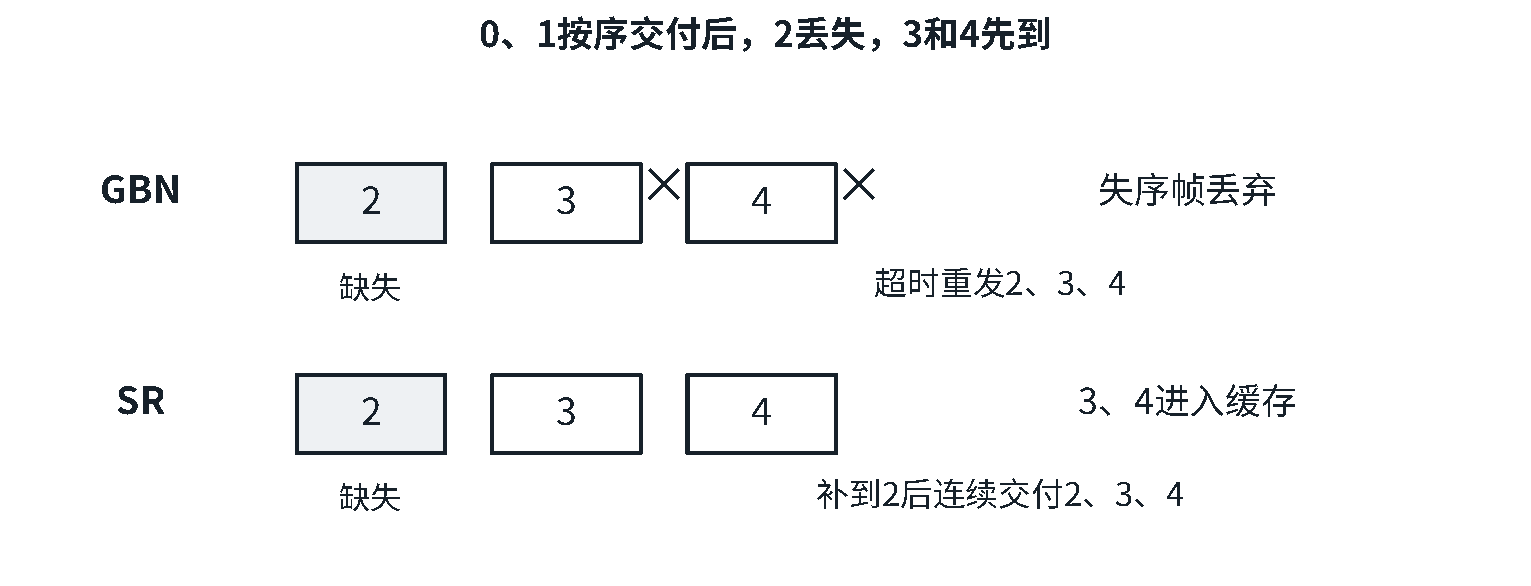
\includegraphics[width=\linewidth,height=125mm,keepaspectratio]{figures/CN04_gbn_sr.pdf}
\captionof{figure}{2号帧丢失后，GBN丢弃后续失序帧，SR缓存后等待补齐}\label{cn-fig-arq}
\end{minipage}\par\medskip

例如发送窗口与接收窗口均为4，编号空间为0～7。0～3发出后，0、1、3已确认而2未确认，发送窗口左沿只能到2，可覆盖2～5；其中3已确认，4、5可新发。接收端若已缓存3，2到达后可连续交付2、3，才把接收窗口推进到4。SR不会因为ACK3出现就把ACK2也当作已收到。

为避免接收窗口把旧一轮重传误当成新帧，需 \(W_s+W_r\le2^k\)；常见对称窗口为 \(W_s=W_r\le2^{k-1}\)。例如5位序号、对称最大窗口为16，不是31；4位序号且 \(W_r=7\) 时，仅由一般不重叠条件得到 \(W_s\le9\)，不能无条件用``半个序号空间''代替不对称条件。王道书§3.4中这两类设问应分别判断。

主书与课件还对常用配置采用 \(W_r\le W_s\)，以免接收窗口大于发送窗口时，多出的部分没有对应新帧、白白占用窗口额度。题目若采用这套教材配置，应同时满足不重叠条件；不能只验证两窗之和就断言任意配置都符合该题模型。上例取 \(W_s=9,W_r=7\) 同时满足这两项，最大对称配置则两窗都取8。

序号空间相同，不意味着 SR 的最大利用率一定超过 GBN。3位序号时 GBN最大发送窗口7，对称SR为4；无差错时若只有窗口约束，GBN可能更容易填满链路。SR的优势在于有差错时能保留已正确收到的失序帧，减少重传；并非任何条件下发送窗口都更大。

把三种ARQ放在同一组条件下比较，关键是确认覆盖范围、失序缓存和超时后的动作。以下沿用本章``ACK i确认已收到i号帧''的约定，序号共 \(k\) bit。

\begin{wideblock}

\par\medskip\noindent\begin{minipage}{\linewidth}\fontsize{9.3}{12}\selectfont\begin{tabularx}{\linewidth}{@{}YYYY@{}}
\toprule\noalign{}
\begin{minipage}[b]{\linewidth}\raggedright
比较维度
\end{minipage} & \begin{minipage}[b]{\linewidth}\raggedright
停止---等待
\end{minipage} & \begin{minipage}[b]{\linewidth}\raggedright
GBN
\end{minipage} & \begin{minipage}[b]{\linewidth}\raggedright
SR
\end{minipage} \\
\midrule\noalign{}


发送/接收窗口 & \(W_s=W_r=1\) & \(W_r=1\)，\(W_s\le2^k-1\)；取1时退化为停等 & \(W_s+W_r\le2^k\)；本书常用 \(W_r\le W_s\)；对称时各不超过 \(2^{k-1}\) \\
确认的含义 & 确认当前帧 & 累计确认按序收到的帧 & 分别确认每个正确接收帧 \\
缺口后的正确帧 & 尚未发送下一新帧 & 失序到达通常丢弃 & 在接收窗口内缓存，补齐缺口后连续交付 \\
超时重传范围 & 当前未确认帧 & 从最早未确认帧起的全部已发未确认帧 & 相应超时未确认帧 \\
典型计时与接收存储 & 一个未确认帧的计时 & 通常计时最早未确认帧；不缓存后续失序帧 & 各未确认帧分别计时；须存储失序帧 \\
\bottomrule\end{tabularx}
\end{minipage}\par\medskip

\end{wideblock}

窗口都以\textbf{帧数}计，不能直接代入TCP的字节窗口。停等牺牲流水换取简单状态；GBN用累计确认和简单接收端降低管理开销；SR增加缓存与计时状态以减少差错后的重复传送。无差错、小窗口、长传播或高误码等条件改变时，比较结论也会改变。

\section{频分、时分、波分与码分怎样共享介质}\label{CN03-09}

频分多路复用 FDM 把频带划成互不重叠的子带，多个用户可同时发送；时分 TDM 把时间划成重复时隙，各用户按时隙使用；波分 WDM 以不同光波长承载不同信号，可视为光频域复用。同步TDM分到的时隙在用户无数据时也可能空着；统计时分按实际有数据的用户动态分配，需要说明数据归属和排队规则。

码分 CDMA 用不同码片序列区分用户。按本节理想同步、等功率、正交模型，把比特1映射为本用户码片 \(c\)，比特0映射为 \(-c\)，未发送为0。多用户信号按码片位置相加；接收者对目标码 \(c\) 做内积并除以码长 \(m\)。正交的其他用户内积为0，目标值为+1、\ensuremath{-}1或0，分别表示1、0或未发送。该结论依赖码序列、同步及功率假设；把任意非正交码直接代入，不能指望干扰仍完全消失。

\subsection{例 3-7　CDMA 先按码片分组，再做内积}\label{CN03-ex7}

{\tcbset{SNbase/.append style={breakable=false}}\begin{example}[配套例题]

配套例题。 站点 A、B、C通过 CDMA 共享链路，A、B、C的码片序列分别是 \texttt{(\allowbreak{}1,\allowbreak{}1,\allowbreak{}1,\allowbreak{}1)\allowbreak{}}、\texttt{(\allowbreak{}1,\allowbreak{}−1,\allowbreak{}1,\allowbreak{}−1)\allowbreak{}} 和 \texttt{(\allowbreak{}1,\allowbreak{}1,\allowbreak{}−1,\allowbreak{}−1)\allowbreak{}}。若 C 从链路上收到的序列是 \texttt{(\allowbreak{}2,\allowbreak{}0,\allowbreak{}2,\allowbreak{}0,\allowbreak{}0,\allowbreak{}−2,\allowbreak{}0,\allowbreak{}−2,\allowbreak{}0,\allowbreak{}2,\allowbreak{}0,\allowbreak{}2)\allowbreak{}}，则 C 收到 A 发送的数据是（　）。

A. 000　B. 101　C. 110　D. 111

\end{example}}

\textbf{解析。} 问的是 A 的数据，使用 A 的码，不因接收站是 C 就改用 C 的码。按每4个码片分成三组，与 \texttt{(\allowbreak{}1,\allowbreak{}1,\allowbreak{}1,\allowbreak{}1)\allowbreak{}} 内积后除4，依次为 \(4/4=1\)、\(-4/4=-1\)、\(4/4=1\)，恢复为101，选 \textbf{B}。若不先按码长分组，会把三个比特混成一次判决。

\section{ALOHA 与 CSMA：监听为何不能消除冲突}\label{CN03-10}

纯 ALOHA 允许有数据就发送，冲突后随机重发。若一帧发送时间为 \(T\)，另一帧只要在它开始前后各 \(T\) 的区间内开始发送，就可能重叠，易受冲突的时间跨度为 \(2T\)。时隙 ALOHA 只在统一时隙边界开始，冲突区间缩为 \(T\)。经典泊松负载、等长帧模型下，吞吐量分别为 \(Ge^{-2G}\) 与 \(Ge^{-G}\)，最大值约为 \(1/(2e)\) 与 \(1/e\)；脱离该随机模型，不把这些数值当成任何网络固定可得的效率。

CSMA 在发送前监听载波。1-坚持遇忙持续监听、空闲立即发送；非坚持遇忙随机等一段时间再监听；\(p\)-坚持适用于时隙信道，空闲时以概率 \(p\) 发送，以 \(1-p\) 延后一个时隙再判断。坚持策略描述的是``如何等到机会''，不代表先到者必获公平顺序。

监听只能看到已经传播到本地的信号。A刚开始发出信号，远端B可能仍检测为空闲并开始发送，所以任何这类 CSMA 都不能仅靠``先听''消除传播期间的冲突。遇忙时的动作以及发生冲突后的动作，要分开读题。

\section{CSMA/CD：最短帧与网络跨度的关系}\label{CN03-11}

共享半双工以太网采用载波监听、多路访问与冲突检测。站点一边发送一边检测；发现冲突后停止正常帧的发送，改发强化冲突信号，再随机退避。全双工点到点交换以太网无需争用共享介质，不使用 CSMA/CD；不能把``所有以太网必采用 CSMA/CD''作为前提。

设最远两站单向传播时间为 \(\tau\)。最不利时，远端在A信号将到前开始发送，冲突的影响再传回A，接近 \(2\tau\) 后A才察觉。为保证A还在发送时能检测，必须有

\[\frac{L_{\min}}R\ge2\tau,\qquad L_{\min}\ge2R\tau.\]

若还包含中继器延时，应计入最坏往返路径。提高速率而保留帧长，会减少可允许的传播时间；不是速率越高、可允许的共享网跨度就越大。

\subsection{例 3-8　最短帧缩短后要缩短多少电缆}\label{CN03-ex8}

{\tcbset{SNbase/.append style={breakable=false}}\begin{example}[配套例题]

配套例题。 在一个采用 CSMA/CD 协议的网络中，传输介质是一根完整的电缆，传输速率为1 Gb/s，电缆中的信号传播速度为200000 km/s。若最小数据帧长度减少800 bit，则最远的两个站点之间的距离至少需要（　）。

A. 增加160 m　B. 增加80 m　C. 减少160 m　D. 减少80 m

\end{example}}

\textbf{解析。} 最短发送时间减少 \(800/10^9=0.8\ \mu s\)，这一时间约束的是往返传播时延；允许的单向传播时间减少0.4 μs。距离应至少减少 \(2\times10^8\times0.4\times10^{-6}=80\) m，选 \textbf{D}。漏掉往返关系会误得160 m。

截断二进制指数退避在第 \(n\) 次冲突后，令 \(k=\min(n,10)\)，从整数 \(0\) 至 \(2^k-1\) 中随机取 \(r\)，等待 \(r\) 个争用时间片后重新竞争。10 Mb/s以太网争用时间片为51.2 μs；连续4次冲突，最大退避为 \(15\times51.2=768\ \mu s\)；连续11次时指数截断为10，最大为 \(1023\times51.2=52.3776\) ms。这两个计算分别展示未截断与已截断的退避边界。达到规定的重试上限会报告失败，而不是无限指数增大。

\section{CSMA/CA、确认与 NAV：隐藏站等到何时}\label{CN03-12}

无线发送端自身信号远强于接收信号，且不同站点的可听范围不同，不能沿用有线的边发边检测。CSMA/CA采用物理载波监听、虚拟载波监听、帧间间隔和随机退避，尽量减少冲突；接收方对成功收到的单播数据帧发送 ACK。没有收到 ACK，发送方才按协议重试；缺 ACK 也可能是 ACK 本身丢失，不一定证明数据没到。

DIFS用于一般数据竞争，SIFS较短，使 ACK、CTS等属于当前交换的响应获得更高优先权。倒计时遇信道忙时冻结，信道恢复空闲并满足相应间隔后继续，不是每听到忙都把已退避的时间无条件作废。

RTS/CTS是可选的预约机制。A向AP发RTS，AP回复CTS后，A发DATA，AP发ACK，相邻响应间隔为SIFS。隐藏站B可能听不到A，却能听到AP的CTS；它根据持续时间字段设置\textbf{网络分配向量 NAV}，在剩余预约期间推迟竞争。RTS/CTS减少某些长数据冲突损失，但有自身开销，不是所有无线单播必用。

\par\medskip\noindent\begin{minipage}{\linewidth}
\centering
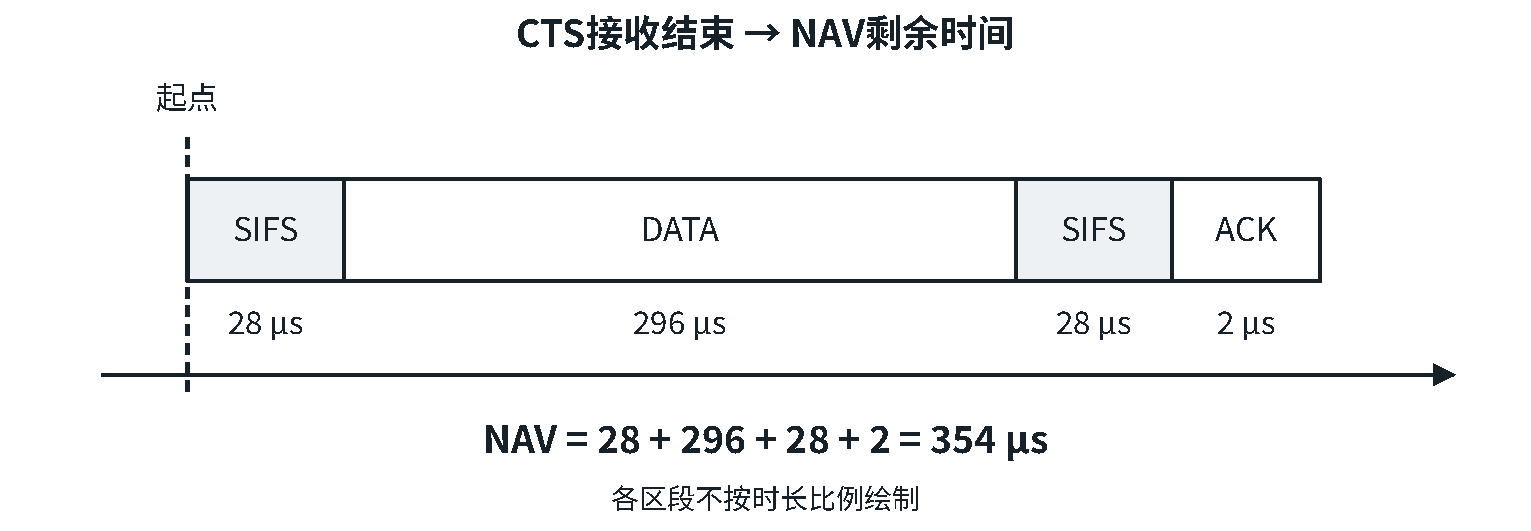
\includegraphics[width=\linewidth,height=125mm,keepaspectratio]{figures/CN05_nav_2024.pdf}
\captionof{figure}{CTS结束后，剩余预约由DATA、ACK及两个SIFS组成}\label{cn-fig-nav}
\end{minipage}\par\medskip

\subsection{例 3-9　收到 CTS 后只计算剩余时间}\label{CN03-ex9}

{\tcbset{SNbase/.append style={breakable=false}}\begin{example}[配套例题]

配套例题。 在采用 CSMA/CA 协议的802.11无线局域网中，DIFS=128 μs，SIFS=28 μs，RTS帧、CTS帧和ACK帧的传输时延分别是3 μs、2 μs和2 μs，忽略信号传播时延。若主机A要向AP发送一个总长度为1998 B的数据帧，无线链路带宽为54 Mb/s，则隐藏站B收到AP发送的CTS帧时，设置的NAV值是（　）。

A. 326 μs　B. 354 μs　C. 385 μs　D. 513 μs

\end{example}}

\textbf{解析。} 起点为CTS已经收到，RTS、前面的DIFS和CTS自身都已经过去。数据发送为 \(1998\times8/54=296\ \mu s\)，余下顺序为 SIFS---DATA---SIFS---ACK，所以

\[NAV=28+296+28+2=354\ \mu s,\]

选 \textbf{B}。图中CTS之前还有一个SIFS，它计入从RTS结束开始预约的区间，不计入收到CTS后的剩余区间。把起点画在时间线上，比直接背``加几个间隔''更可靠。

\section{令牌传递与轮询：如何给出有界的使用机会}\label{CN03-13}

轮询由控制站依次询问各站是否需要发送，避免数据站任意竞争，但控制站、轮询开销与等待次序会影响性能。令牌传递把发送许可放在沿逻辑环传递的控制帧中，获得令牌的站才能发送，发送后按规则释放。

正常运行、只有一个有效令牌的模型下不会发生数据争用冲突；需有机制处理令牌丢失、重复与站点失效。为防止其他站长期等待，站点持有令牌有时间或发送量上限。无数据的站应及时转交令牌，不必把上限时间耗满；有很多数据的站也不能一直占用到全部发完。〖3.5-014〗中的两个绝对说法都忽略了这一约束。重负载下轮流使用可减少反复碰撞，轻负载下则可能多付令牌等待开销。

\section{局域网与 IEEE 802 的层次}\label{CN03-14}

局域网技术通常覆盖物理层与数据链路层。IEEE 802体系把数据链路层进一步划为逻辑链路控制 LLC 与介质访问控制 MAC，MAC负责与具体介质有关的寻址、成帧和访问控制等工作。网卡通常同时实现物理信号收发与链路层帧处理，不能因为``用 MAC 地址''便认为它没有物理层功能。〖3.6-004〗〖3.6-023〗

以太网、无线局域网可采用不同MAC机制，仍可在网络层共同承载IP。MAC地址只在适用的链路技术和广播范围内有意义，交换机学习的目的不是建立全互联网的MAC路由表。

\section{以太网帧、MAC 地址与有效载荷}\label{CN03-15}

本节采用\textbf{Ethernet II，即DIX Ethernet V2、无VLAN标签}的格式。MAC帧从目的地址起依次为目的MAC 6 B、源MAC 6 B、类型2 B、数据及必要填充46～1500 B、FCS 4 B。前3个字段组成\textbf{14 B MAC帧头}；帧头、数据/填充与FCS一起才是完整MAC帧，长度为64～1518 B。FCS是帧尾，不能把首尾共18 B都称为首部。

\par\medskip\noindent\begin{minipage}{\linewidth}
\centering
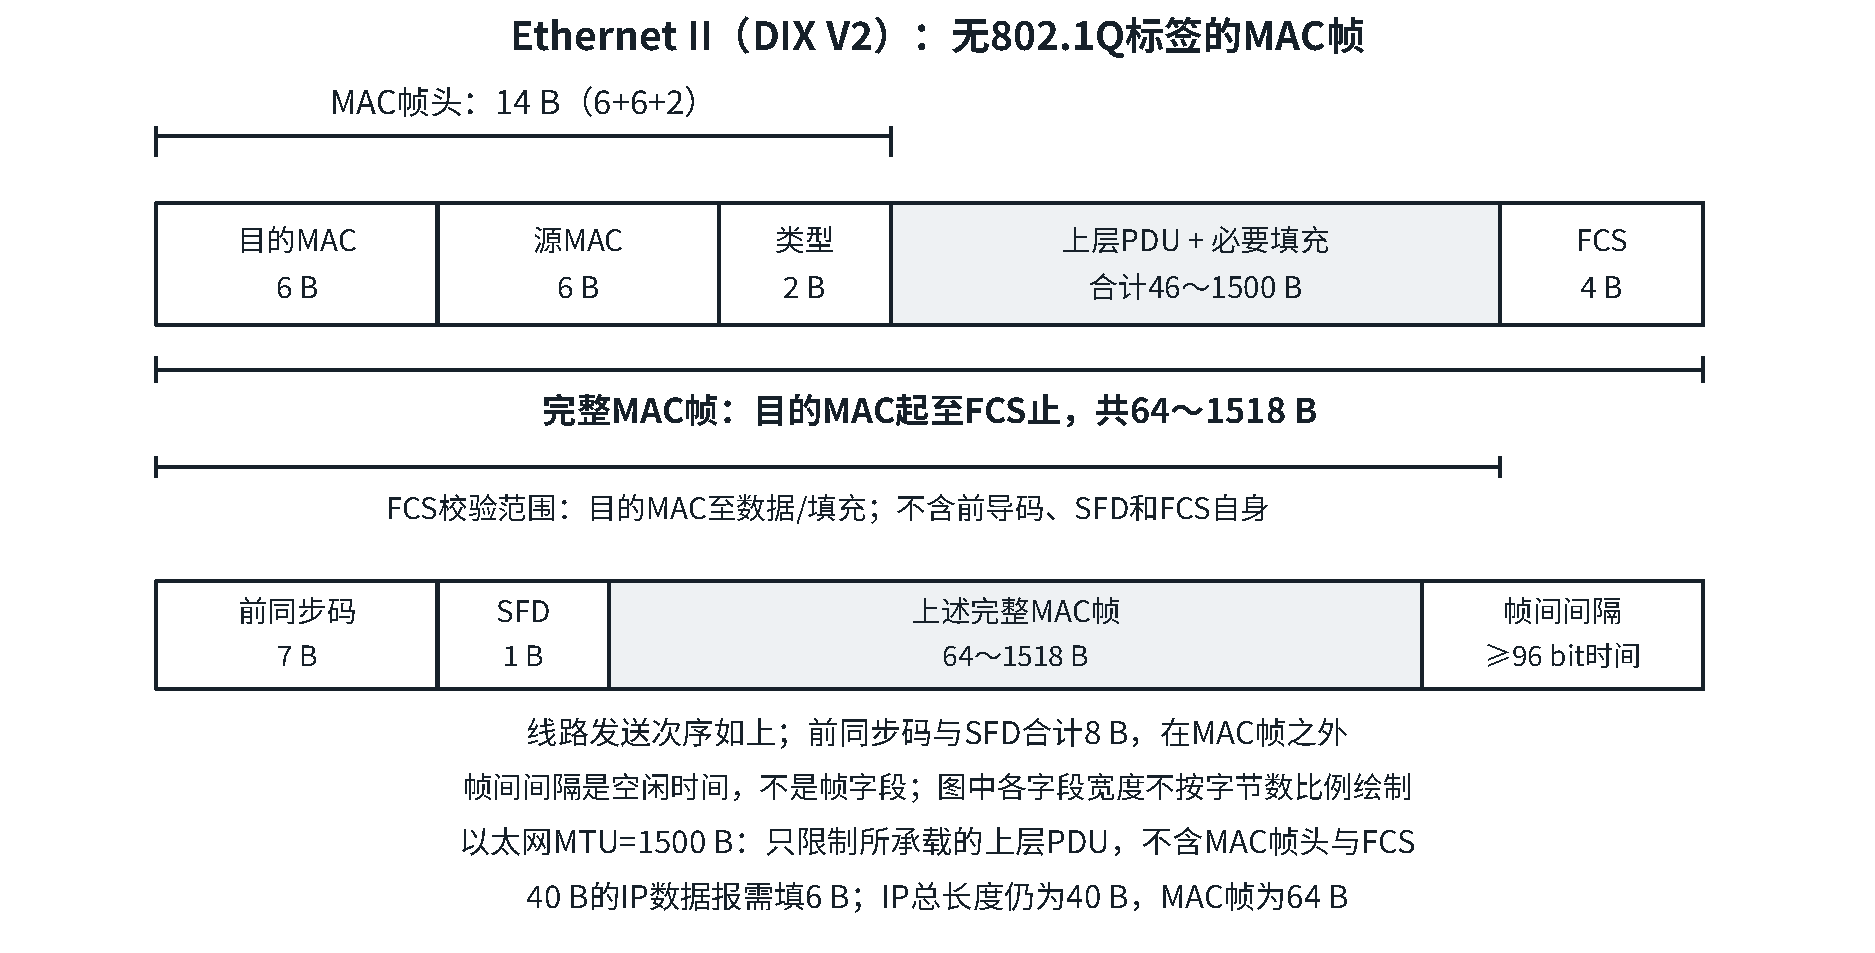
\includegraphics[width=\linewidth,height=125mm,keepaspectratio]{figures/CN19_ethernet_frame.pdf}
\captionof{figure}{Ethernet II无标签帧：帧头14 B，MAC帧64～1518 B；前同步码、SFD与帧间间隔另计}\label{cn-fig-ethernet-format}
\end{minipage}\par\medskip

线路在MAC帧前另发送7 B前同步码和1 B帧开始定界符SFD，二者常合称8 B前导部分，用于同步与开始定界，均不计入上述MAC帧长。帧间间隔至少为96 bit的发送时间，它是空闲时间而不是帧字段。10 Mb/s时相当于9.6 μs；若只将这项时间折算成字节的发送时间，相当于12 B，但线上并没有因此再增加一个12 B帧字段。

类型字段说明承载的上层协议，例如 \texttt{0x0800} 表示IPv4、\texttt{0x0806} 表示ARP。IEEE 802.3的基本格式在同一位置使用长度字段，不能把它和Ethernet II的类型字段同时算成两个独立字段。两种格式的区别不改变本节无标签MAC帧的源、目的各6 B与FCS 4 B口径。

MAC地址通常48 bit，以6组十六进制表示。目的全1是广播地址；首字节最低位指示单播与组播。源地址标识发送该帧的接口，一般不能填成广播地址。以太网FCS使用CRC，只检查当前帧；错误帧通常丢弃，以太网MAC不负责确认重传。

FCS占32 bit，发送端对从目的MAC到数据末尾（含必要填充）的比特计算CRC，接收端按对应规则检验；前同步码、SFD、帧间间隔不参加该MAC帧校验。以太网MTU=1500 B限制的是所承载的上层PDU，如完整IP数据报，不包括14 B帧头和4 B FCS。因而``IP总长度1500 B''和``以太网MAC帧1518 B''描述的是同一次封装的不同边界。

一个40 B的IP数据报装入普通无标签帧，需要填充6 B。IP总长度仍写40 B，填充属于以太网帧数据区，接收IP层依据自己的长度字段取出数据，不把填充当成IP载荷。以太网以帧作为传送/交换单位，属于分组交换技术，不能因为有``交换机''就推断为电路交换。〖3.6-003〗

计算效率要先确定分母范围。若只问MAC帧内应用数据效率，用应用字节数除MAC帧长；若问线上连续发送的有效吞吐量，还可能需要加入前导码与帧间间隔。吉比特与更高速以太网的物理编码各有制式，不能把10 Mb/s的曼彻斯特编码直接套用到更高速率。

例如连续发送最短帧，若题目明确计入8 B前导部分及96 bit时间的间隔、忽略物理编码额外开销，一个周期为 \((8+64)\times8+96=672\) bit时间，即84 B的发送时间。64 B对应的是MAC帧长，84 B对应的是这一模型下每帧占用的周期；两者分母不同，不能互换。最短MAC帧长的规则也继续适用于普通全双工帧，不能因为不使用CSMA/CD就删去必要填充。

\section{802.11：接收者、发送者和原始端点可能不同}\label{CN03-16}

基础设施无线局域网由接入点 AP 与相关联站点形成基本服务集 BSS，AP的无线接口地址用作BSSID。多个BSS经分布式系统互联可组成扩展服务集；站点移动时可重新关联。AP负责无线接入及桥接，不因名为``接入点''就自动具有跨子网路由功能。

无线帧常需要同时记录当前无线跳的收发接口和原始源/目的。常见三地址数据帧可按下表判断；这里DS表示分布式系统。

\begin{wideblock}

\par\medskip\noindent\begin{minipage}{\linewidth}\fontsize{9.3}{12}\selectfont\begin{tabularx}{\linewidth}{@{}YYY@{}}
\toprule\noalign{}
方向与控制位 & 地址1、地址2 & 地址3 \\
\midrule\noalign{}


站点\ensuremath{\to}AP，ToDS=1、FromDS=0 & 当前接收者AP、当前发送站点 & 最终目的MAC \\
AP\ensuremath{\to}站点，ToDS=0、FromDS=1 & 当前接收站点、当前发送者AP & 原始源MAC \\
同一自组织网，二位均0 & 目的、源 & BSSID \\
\bottomrule\end{tabularx}
\end{minipage}\par\medskip

\end{wideblock}

两位都为1的无线分布式转发可能使用第四地址，不能把三地址表硬套过去。A经过AP1、有线分布式系统、AP2转发给B时，在AP2\ensuremath{\to}B这一无线跳上，地址1=B、地址2=AP2的BSSID、地址3=原始A；AP1不是该跳的发送接口。〖3.6-031〗考查的正是这个端点区分。

以太网与无线局域网都可承载IP，但应在相同介质条件下比较访问和交付机制。

\begin{wideblock}

\par\medskip\noindent\begin{minipage}{\linewidth}\fontsize{9.3}{12}\selectfont\begin{tabularx}{\linewidth}{@{}YYYY@{}}
\toprule\noalign{}
\begin{minipage}[b]{\linewidth}\raggedright
比较维度
\end{minipage} & \begin{minipage}[b]{\linewidth}\raggedright
共享半双工以太网
\end{minipage} & \begin{minipage}[b]{\linewidth}\raggedright
交换全双工以太网
\end{minipage} & \begin{minipage}[b]{\linewidth}\raggedright
本章802.11 DCF无线模型
\end{minipage} \\
\midrule\noalign{}


发送机会 & 多站共享，使用CSMA/CD竞争 & 每条点到点链路可同时双向发送，无CSMA/CD竞争 & 共享无线信道，使用CSMA/CA与退避 \\
冲突怎样处理 & 发送中检测，发现后中止并退避 & 正常全双工链路没有传统共享介质冲突 & 难以可靠边发边检测；用监听、预约及反馈减少损失 \\
基本链路确认 & 无逐帧MAC确认重传 & 无逐帧MAC确认重传 & 普通单播数据帧成功后ACK，必要时重试；广播/组播不套用此ACK流程 \\
地址的判断 & 当前以太网帧的源与目的 & 当前以太网帧的源与目的 & 还要区分当前收发接口、原始端点及DS方向位 \\
\bottomrule\end{tabularx}
\end{minipage}\par\medskip

\end{wideblock}

无线ACK与TCP ACK所在层次、确认单位和作用范围不同。即使当前无线帧已确认，后续网络仍可能丢失IP分组；反过来，没有无线ACK也可能是ACK丢失。比较时应先指出反馈来自哪一层，再决定重传谁。

\section{VLAN：广播域如何跨交换机延伸}\label{CN03-17}

VLAN把一个交换网络划成多个逻辑广播域。一个VLAN中的广播只在该VLAN允许的端口传播；不同VLAN之间的IP通信需要路由等三层功能。VLAN不等于链路聚合，前者划分逻辑广播范围，后者把多条链路组成一条逻辑连接。安全性改善也取决于正确配置，不能把VLAN当成所有攻击的隔离保证。

接入口常给主机提供无标签帧，交换机根据端口配置确定所属VLAN；交换机之间的干道可携带多个VLAN，使用802.1Q标签标识归属。因此同一VLAN可以跨多台交换机，不要求主机发送的每一帧都自带标签。

802.1Q在源地址之后插入4 B标签，其中含TPID和标签控制信息，VID占12 bit；可编码4096个数值，但0、4095有保留用途，通常可配置的普通VLAN ID为1～4094。含单个标签的常见最大MAC帧长度由1518 B变为1522 B，原FCS应相应更新，不能要求增加标签却保持最大长度不变。〖3.6-032〗

\subsection{例 3-10　填充前先识别有无标签}\label{CN03-ex10}

{\tcbset{SNbase/.append style={breakable=false}}\begin{example}[配套例题]

〖3.6-008〗 一个长度为40 B的IP数据报需要封装成802.1Q帧进行传输，则此802.1Q帧的数据载荷部分需要填充的字节数是（　）。

A. 2　B. 4　C. 6　D. 8

\end{example}}

\textbf{解析。} 本题按王道书的计量模型：含标签MAC帧最短仍按64 B计，首尾部共 \(6+6+4+2+4=22\) B，数据区下限为42 B。因而需填充 \(42-40=2\) B，选 \textbf{A}。若采用前节普通无标签帧，首尾部18 B、数据区下限46 B，同一个IP数据报会填6 B。不要混用两套字段长度；实际设备插入标签时原有填充是否保留，是另一项处理规则。

\section{广域链路与 PPP：不需要争用不等于没有成帧}\label{CN03-18}

广域网侧重把较远节点互连，核心常由路由器和点到点链路组成；具体设备和传输协议不必与某一种局域网相同。PPP在点到点链路上封装网络层分组，不必解决多站争用，因此不使用CSMA/CD，也没有按争用时间片规定的64 B最小帧要求。

PPP常见基本帧依次为标志 \texttt{7E}、地址 \texttt{FF}、控制 \texttt{03}、协议字段、信息字段、FCS、标志 \texttt{7E}。协议字段区分IP、LCP或某一NCP等。LCP负责建立、配置与测试数据链路，NCP是一组针对不同网络层协议的配置协议；LCP建立不等于已经取得IP通信所需的全部配置。

异步PPP使用字节转义，例如将数据 \texttt{7E} 发送为 \texttt{7D 5E}，\texttt{7D} 发送为 \texttt{7D 5D}；接收端逆向恢复。教材同步PPP模型采用零比特填充。PPP以FCS检错，基本协议不靠数据帧编号和确认重传来提供可靠交付；不能因名称中``协议''或连接曾建立便认定它必可靠。

\section{交换机如何学习、过滤和转发}\label{CN03-19}

交换机收到帧后，先根据\textbf{源MAC地址与入端口}学习或更新表项，再查\textbf{目的MAC地址}决定出口。若目的表项在另一端口，定向转发；若目的表项就在入端口，过滤；若目的未知或是广播，在当前VLAN内除入端口外的允许端口泛洪。学习表项时不能从目的地址反推其位置，因为帧可能正是由于目的未知才发来。

\par\medskip\noindent\begin{minipage}{\linewidth}
\centering
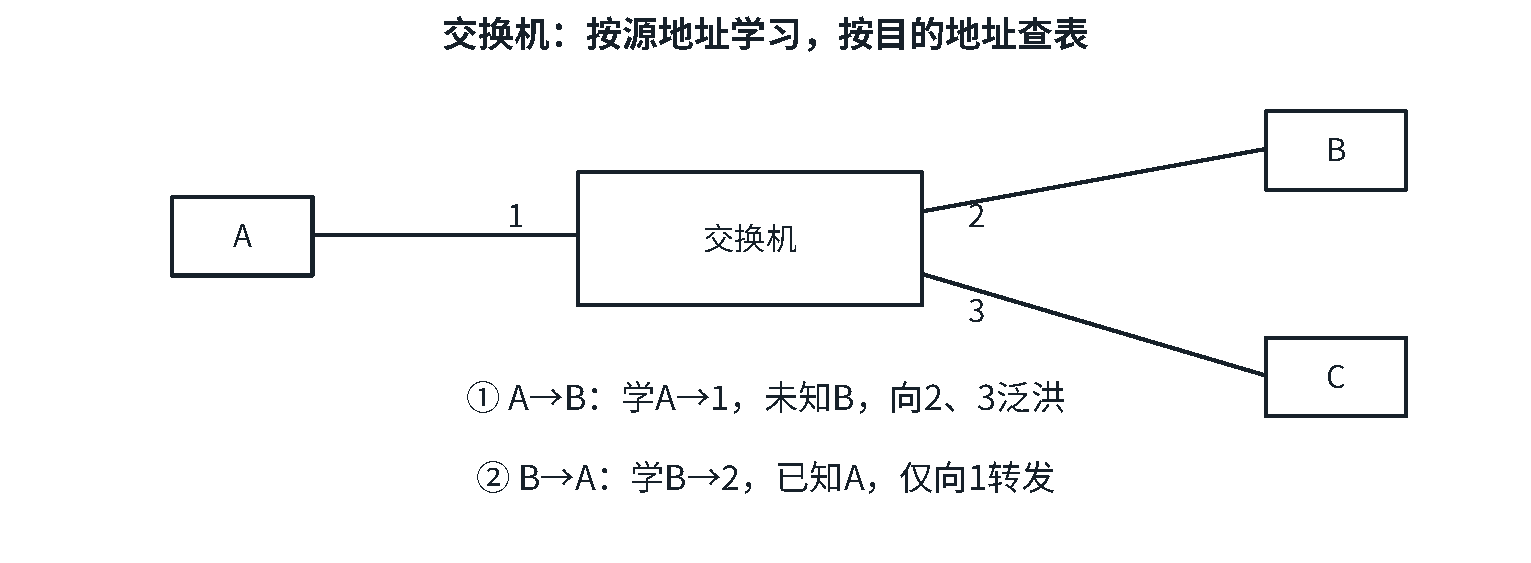
\includegraphics[width=\linewidth,height=125mm,keepaspectratio]{figures/CN06_switch_learning.pdf}
\captionof{figure}{首次A\ensuremath{\to}B使交换机学习A；B回复时定向转发并学习B}\label{cn-fig-switch}
\end{minipage}\par\medskip

图中转发表初始为空。A由端口1发给B，交换机记 \texttt{A→1}，向2、3泛洪；B从端口2回复A，记 \texttt{B→2}，查A只向1转发。若以后端口1上的另一站发来目的为A的帧，交换机查出目的也在1，就不再向其他端口转发。表项会老化，拓扑有环还需要生成树等机制避免广播持续循环。

交换机各端口可形成独立冲突域，普通二层交换机不因端口不同自动隔离广播域；VLAN配置另行划分广播域。全双工独立链路上本来就不发生传统共享介质冲突，``每端口一冲突域''是题目常用的拓扑比较口径，不等于每条全双工链路都有实际碰撞。

\subsection{例 3-11　直通交换最早何时能决定出口}\label{CN03-ex11}

{\tcbset{SNbase/.append style={breakable=false}}\begin{example}[配套例题]

配套例题。 对于100 Mb/s的以太网交换机，当输出端口无排队，以直通交换方式转发一个以太网帧（不包括前导码）时，引入的转发时延至少是（　）。

A. 0 μs　B. 0.48 μs　C. 5.12 μs　D. 121.44 μs

\end{example}}

\textbf{解析。} 直通交换不必收全帧，但至少需要读完位于帧开头的6 B目的地址，才能作转发决策。时间为 \(6\times8/(100\times10^6)=0.48\ \mu s\)，选 \textbf{B}。5.12 μs是接收64 B所需时间，属于另一种等待情形；题目已明确不计前导码，也不要再增加8 B。

存储转发要收齐帧并能完成FCS检查后才转发；直通在帧尾未到前便可能开始，降低转发等待，却不能预先排除帧尾才发现的错误。总吞吐量题还要明确统计发送量还是收发之和。独立端口可以并行，但经过同一低速出口的流仍共享那个瓶颈；把11个端点都写成100 Mb/s之前，应检查是否真能安排不超端口能力的通信。

\subsection{例 3-12　双向 GBN：确认号、回绕与重传要分开追踪}\label{CN03-ex12}

{\tcbset{SNbase/.append style={breakable=false}}\begin{example}[配套例题]

配套例题。 甲乙双方均采用后退 N 帧协议（GBN）持续进行双向数据传输，始终采用捎带确认，帧长均为1000 B。\(S_{x,y}\)、\(R_{x,y}\)分别表示甲方、乙方发送的数据帧，\(x\)为发送序号，\(y\)为确认序号，表示希望接收对方的下一帧序号。两个序号字段均为3 bit，信道传输速率为100 Mb/s，RTT=0.96 ms。下图为甲方发送和接收数据帧的两种场景；\(t_0\)时甲方的发送序号和确认序号均为0，\(t_1\)时甲方有足够多的数据待发送。

\par\medskip\noindent\begin{minipage}{\linewidth}
\centering
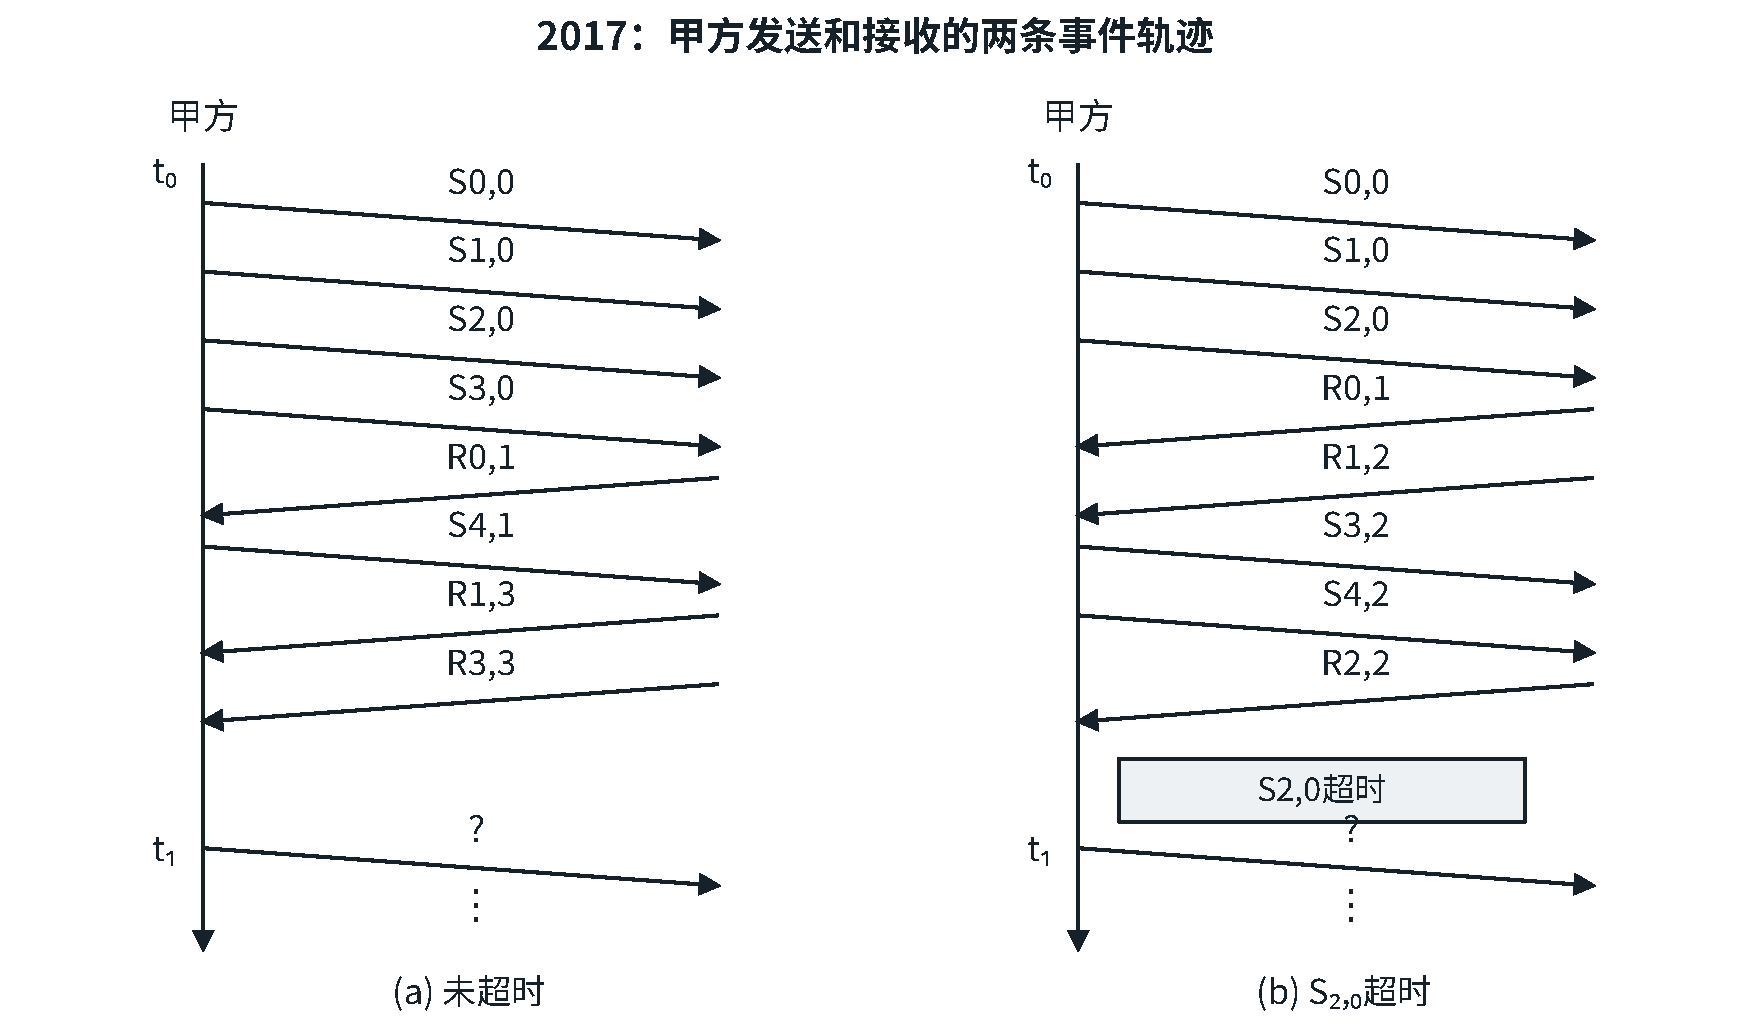
\includegraphics[width=\linewidth,height=125mm,keepaspectratio]{figures/CN20_gbn_2017.pdf}
\captionof{figure}{箭头从甲方发出为S、指向甲方为R；两列分别对应未超时和S2,0超时的原题场景}\label{cn-fig-gbn2017}
\end{minipage}\par\medskip

（1）对于图(a)，\(t_0\)到\(t_1\)期间，甲方可以断定乙方已正确接收多少个数据帧？是哪几个帧？请用\(S_{x,y}\)表示。

（2）对于图(a)，从\(t_1\)起，在不出现超时且未收到乙方新的数据帧之前，甲方最多还可以发送多少个数据帧？第一个和最后一个分别是什么？请用\(S_{x,y}\)表示。

（3）对于图(b)，从\(t_1\)起，在不出现新的超时且未收到乙方新的数据帧之前，需要重发多少个数据帧？重发的第一个帧是什么？请用\(S_{x,y}\)表示。

（4）甲方可以达到的最大信道利用率是多少？

\end{example}}

\textbf{解析。} 读题时先分清两条状态线：收到帧的确认序号决定``我发出的哪些帧已被确认''；收到帧的发送序号决定``我下次应捎带哪个确认号''。GBN的接收窗口为1，收到失序帧不能跳过缺口向前确认。序号空间为\(2^3=8\)，发送窗口最多为7，所有序号按模8回绕。

图(a)最后收到\(R_{3,3}\)。其确认号3累计确认甲方序号0、1、2已正确到达，因此第（1）问为3帧：\(S_{0,0}\)、\(S_{1,0}\)、\(S_{2,0}\)。不能因它的发送序号为3，便推断甲方也收齐了乙方0～3号帧：甲方依次正确收到\(R_{0,1}\)、\(R_{1,3}\)，随后缺少乙方2号帧，\(R_{3,3}\)作为失序帧被丢弃，所以甲方仍希望收到乙方2号帧。

此时甲方已发送到\(S_{4,1}\)，未确认的是发送序号3、4两帧。7个窗口位置中还剩\(7-2=5\)个；下一发送序号从5开始，捎带确认号始终为2，故第（2）问可发送\(S_{5,2}\)、\(S_{6,2}\)、\(S_{7,2}\)、\(S_{0,2}\)、\(S_{1,2}\)，首帧为\(S_{5,2}\)，末帧为\(S_{1,2}\)。回绕后的0、1是新一轮数据，不能与已经确认的旧0、1混为一谈。

图(b)乙方最后通告确认号2，意味着甲方0、1号已确认，2、3、4号仍未确认。\(S_{2,0}\)超时触发从最早未确认帧开始的后退重传，因此第（3）问重发3帧。甲方此时已按序收到乙方\(R_{2,2}\)，期待乙方下一帧为3，故重传首帧应更新捎带确认号，写成\(S_{2,3}\)；随后为\(S_{3,3}\)、\(S_{4,3}\)，不能照抄旧帧的确认号0。

第（4）问须保留捎带确认帧的发送时间。发送一个数据帧需\(T_d=1000\times8/(100\times10^6)=0.08\) ms；确认也装在1000 B的数据帧中，\(T_a=0.08\) ms。沿用教材模型：题目中的RTT表示往返传播时延；从发送首帧到完整收到其确认，周期为\(T_d+\mathrm{RTT}+T_a=1.12\) ms。最多连续发7帧，故\(U_{\max}=7\times0.08/1.12=50\%\)。全双工允许两个方向同时工作，但本题求甲方单方向利用率；也不能把长捎带确认当成长度可忽略的纯ACK。

\section{主动回忆自测}\label{CN03-review}

以下为自拟题。先说明所用ACK语义、序号空间与链路模型，再回答。

\begin{enumerate}
\def\labelenumi{\arabic{enumi}.}
\tightlist
\item
  数据\texttt{111110}按零比特填充后是什么？去填充时删除几个0？
\item
  3位序号下，GBN最大发送窗口与对称SR最大窗口分别是多少？
\item
  SR接收窗口为2～5，已缓存3、4，随后收到2。哪些帧可按序交付？
\item
  A、B、C、D接入普通无VLAN交换机的四个全双工端口，能同时A\ensuremath{\to}B和C\ensuremath{\to}D吗？是否自动成为两个广播域？
\item
  CRC余数为0，能否证明所有可能的传输错误都未发生？码距4能保证检测、纠正多少位错？
\item
  为什么共享半双工以太网最短帧必须持续发送至少一个最坏往返传播时间？
\item
  收到CTS以后设置NAV，是否应把已经过去的RTS和CTS发送时间再算一次？
\item
  一个40 B IP数据报装进普通无VLAN的Ethernet II帧，至少填多少字节？IP总长度字段会跟着增大吗？
\item
  交换机收到从A发向未知B的帧，应从源地址还是目的地址学习端口？PPP是否需要CSMA/CD？
\end{enumerate}

\subsection{核对答案}\label{CN03-review-answers}

\begin{enumerate}
\def\labelenumi{\arabic{enumi}.}
\tightlist
\item
  \texttt{1111100}，删除第五个1后插入的0，保留原数据末尾的0。
\item
  7和4；一般SR约束是两窗和不超过序号空间，对称时才直接取一半。
\item
  连续交付2、3、4，左沿移到5，不能越过还缺的5。
\item
  可以，两个流的输出端口不同；仍是一个广播域，隔离广播需相应VLAN或三层边界。
\item
  不能，存在非零错误模式被生成式整除；码距4可保证检出3位错、纠正1位错。
\item
  让最远端最晚产生的冲突反馈返回时，发送站仍在发送，才能检测到冲突。
\item
  不应，NAV描述当前时刻之后的剩余预约区间。
\item
  填6 B；IP总长度仍为40 B，填充属于链路封装。
\item
  学源地址A与入端口，目的B未知时在当前VLAN内泛洪；点到点PPP无需多站争用，因而不使用CSMA/CD。
\end{enumerate}
